\documentclass[twoside]{article}
\usepackage[T1]{fontenc}
\usepackage[utf8]{inputenc}
\usepackage[magyar]{babel}
\usepackage[margin=3cm]{geometry}
\usepackage{amsmath,amssymb,tikz,fancyhdr,commath}

\usetikzlibrary{shapes,decorations.pathreplacing,arrows}

\title{Mérési jegyzőkönyv\\
\large Forgási energia mérése, tehetetlenségi nyomaték számítása}
\author{Horváth Dávid}

\fancyhead[LE,RO]{Mérési jegyzőkönyv}
\fancyhead[RE,LO]{Horváth Dávid}

\begin{document}
\pagestyle{fancy}
\maketitle
\tableofcontents
\pagebreak
\section{Elméleti háttér}
	A lejtőn leguruló henger összetett mozgást végez, mivel halad, és forog is egyidőben. 
	\subsection{Haladó mozgás}
	A haladó mozgásra, mivel a lejtőn egyenletesen gyorsuló mozgást végez, a következő összefüggéseink vannak:
	\begin{gather}
		v(t)=v_0*t+\frac{a}{2}*t^2\label{eq:1}\\
		s=\frac{v(t)+v_0}{2}*t\label{eq:2}
	\end{gather}
	\subsection{Forgómozgás}
		A forgómozgás egy kiterjedt merev test rögzített tengely körüli forgása. 
		\subsubsection{Kinematika}
			Kinematikai leírása a következő mennyiségekkel történhet, a körmozgáshoz hasonlóan:
			\begin{enumerate}
				\item Periódusidő\\
					jele T\\
					$[T]=s$
				\item Fordulatok száma (frekvencia)\\
					jele f\\
					$[f]=\frac{1}{s}$
				\item Szögelfordulás\\
					jele $\varphi$\\
					$[\varphi]=$rad
				\item Szögsebesség\\
					jele $\omega$\\
					$[\omega]=\frac{1}{s}$
				\item Kerületi sebesség\\
					jele $v_k$\\
					$[v_k]=\frac{m}{s^2}$
				\item Szöggyorsulás\\
					jele $\beta$\\
					$[\beta]=\frac{1}{s^2}$
				\item Centripetális gyorsulás\\
					jele $a_{cp}$\\
					$[a_{cp}]=\frac{m}{s^2}$
				\item Tangenciális gyorsulás\\
				 	jele $a_{tang}$\\
				 	$[a_{tang}]=\frac{m}{s^2}$
			 	\item Eredő gyorsulás\\
			 		jele $a_e$\\
			 		$[a_e]=\frac{m}{s^2}$
			\end{enumerate}
			\pagebreak
			Ezen mennyiségek között az alábbi összefüggések léteznek:
			\begin{gather}
				v_k=r*\omega\label{eq:3}\\
				a_{cp}=\frac{v_k^2}{r}=\omega^2*r\label{eq:4}\\
				a_{tang}=v_k'(t)=r*\beta\label{eq:5}\\
				a_e=\sqrt{a_{cp}^2+a_{tang}^2}\label{eq:6}
			\end{gather}
		\subsubsection{Dinamika}
			Amennyiben a testen forgatónyomaték keletkezik, azaz olyan erő hat rá, amely nem megy át a tömegközéppontján a forgás szögsebessége nőni kezd. Ezt a forgatónyomatékot az $M=F*k$ képlettel számolhatjuk, ahol M a forgatónyomaték, F az erő, k az erőkar.
			
			Amennyiben M állandó, $\beta$ egyenletesen változik, így $M\sim\beta$, azaz $\frac{M}{\beta}$ állandó, ez a hányados a tehetetlenségi nyomaték, jele $\Theta$:
			\begin{gather}
				\frac{M}{\beta}=\Theta\label{eq:7}\\
				[\Theta]=kg\ m^2\label{eq:8}
			\end{gather}
			Ez egy skalármennyiség, ami az adott merev testre jellemző állandó, tömeg, tömegeloszlás, és forgástengely határozza meg:
			\begin{equation}
				\sum_{i=1}^{\infty} m_i*r_i^2\label{eq:9}
			\end{equation}
			Ahol $m_i$ egy tömegpont tömege, $r_i$ a forgástengelytől mért távolsága. Amennyiben a \eqref{eq:7} egyenletet átrendezzük a dinamika alapegyenletéhez hasonlót kapunk:
			\begin{equation}
				M=\Theta*\beta\label{eq:10}
			\end{equation}
			Amit a forgómozgás alapegyenletének nevezünk.
		\subsubsection{Perdület}
			Definiáljuk a perdületet a lendülethez hasonlóan: 
			\begin{equation}
				N=\Theta*\omega\label{eq:11}
			\end{equation}
		 	ahol N a perdület, mértékegysége: $\frac{kg*m^2}{s}$. A forgómozgás alapegyenletéből:
			\begin{align}
				\nonumber M&=\Theta\frac{\dif\omega}{\dif t}\\
				M\dif t&=\Theta\dif\omega\label{eq:12}
			\end{align}
			\eqref{eq:11}, és \eqref{eq:12}-ből:
			\begin{align}
				M\dif t&=\dif N\label{eq:13}\\
				M&=N'(t)\label{eq:14}
			\end{align}
			
			A perdületmegmaradás törvénye kimondja, hogy zárt forgó rendszer perdülete állandó, azaz:
			\begin{equation}
				\sum N=\text{állandó}\label{eq:15}
			\end{equation}
			\begin{figure}
				\centering
				\begin{tikzpicture}[scale=1]
					\draw (-2,0) -- (2,0);
					\draw (0,0) -- (0,-3);
					\draw (0,-3) circle (2cm);
					\draw (0,-3) -- (2,-3) node[midway,yshift=-0.5cm]{r};
					\draw (0,-3) -- (1.414,-1.586) node[midway,yshift=0.5cm]{r};
					
					\draw (1.5,-7) rectangle (2.5,-6) node[midway]{m};
					\draw (2,-6) -- (2,-3);
					\draw[thick] (2,-3) arc (0:45:2) node[midway,xshift=0.25cm]{h};
					\draw[dashed] (2.5,-7) -- (4,-7);
					\draw[dashed] (2.5,-9) -- (4,-9);
					
					\draw [decorate,decoration={brace,amplitude=10pt}] 
					(4,-7) -- (4,-9) node[midway,xshift=0.6cm]{h};
					
					\node at (0.4,-2.85) {$\varphi$};
					
					\draw[->] (2,-7) -- (2,-8) node[midway, xshift=0.5cm]{$F_g$};
					\draw[->,thick] (2,-6) -- (2,-5) node[midway, xshift=0.5cm]{$F_k$};
					\draw[->,thick] (2,-4) -- (2,-5) node[midway, xshift=0.5cm]{$F$};
				\end{tikzpicture}
				\caption{Forgási munka}
				\label{fig:1}
			\end{figure}
		\subsubsection{Munka, energia}
			Tekintsük az \ref{fig:1}. ábrát. Mivel tudjuk, hogy $W=F*s$, és $W=m*g*h$, az ábra jelöléseit használva:
			\begin{equation}
				W_f=F*h=F*r*\varphi=M*\varphi\label{eq:16}
			\end{equation}
			Mivel a mozgási energia: $E_m=\frac{m*v^2}{2}$, a \eqref{eq:3} egyenletet használva:
			\begin{equation}
				E_f=\frac{m*\omega^2*r^2}{2}=\frac{\Theta*\omega^2}{2}\label{eq:17}
			\end{equation}
			A haladó mozgásból ismert munkatétel forgási energiára a következőképpen néz ki:
			\begin{equation}
				W_f=\Delta E_f\label{eq:18}
			\end{equation}
	\subsection{Hibaszámítások}
		Mindenhol 95\%-os konfidencia intervallummal számoltam. Először kiszámoltam minden mért érték hibáját. Amelyik adatnál csak egy mérés van, ott hibának az utolsó értékes jegy (digit) felét vettem, ahol több, ott értéknek a mérések átlagát, míg hibának a szórásukat:
		\begin{gather}
			\overline{x}=\frac{\sum_{i=1}^{n} x_i}{n}\label{eq:19}\\
			\sigma_x=t^**\sqrt{\frac{\sum_{i=1}^{n} (x_i-\overline{x})^2}{n(n-1)}}\label{eq:20}
		\end{gather}
		A \eqref{eq:20} egyenletben $t^*$ a t-eloszlás kritikus értéke. Számolt adatoknál a hibát a Gauss-féle hibaterjedési törvény alapján számoltam:
		\begin{equation}
			\Delta f(x_1,x_2,...,x_n)=\sqrt{\sum_{i=1}^{n}\left(\frac{\partial f}
			{\partial x_i}*\Delta x_i\right)^2}\label{eq:21}
		\end{equation}
		Minden egyenletnél közlöm a nemnulla parciális deriváltakat, és ezek értékeit.
\section{Mérés leírása}
	Használt eszközök:
	\begin{itemize}
		\item lejtő
		\item vékony falú henger
		\item tömör henger
		\item mérőszalag
		\item tolómérő
		\item stopper
		\item mérleg
	\end{itemize}
	\begin{figure}\label{fig:2}
		\centering
		\caption{Mérési összeállítás}
		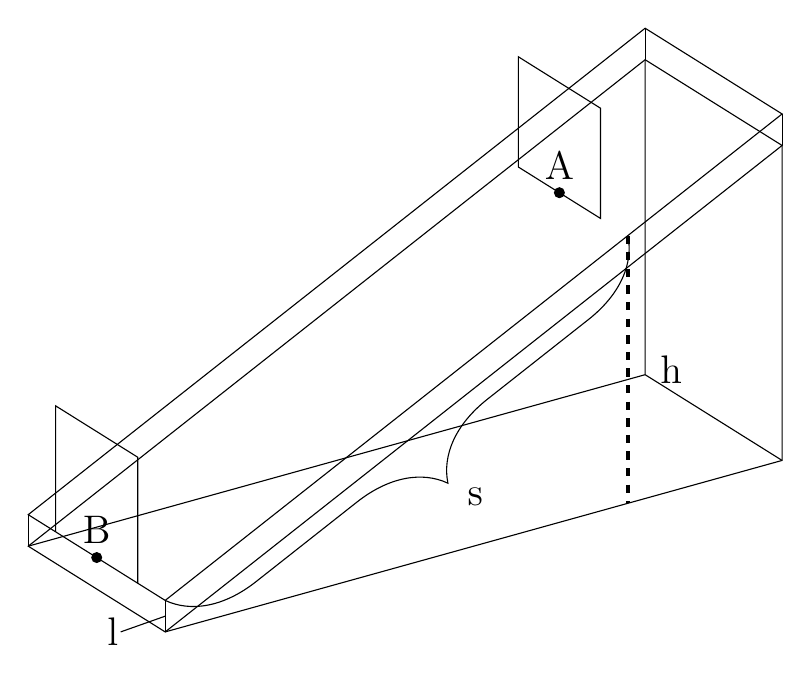
\begin{tikzpicture}[scale=4,rotate around x=90, rotate around z=-45]
			\Large
			\draw (0,0,0) -- (2,0,-1) -- (2,-1,-1) -- (0,-1,0) -- cycle;
			\draw (2,0,-1) -- (2,0,0) -- (0,0,0);
			\draw (2,-1,-1) -- (2,-1,0) -- (0,-1,0);
			\draw (2,-1,0) -- (2,0,0);
			
			\draw (0,0,-.1) -- (2,0,-1.1) -- (2,-1,-1.1) -- (0,-1,-.1) -- cycle;
			\draw (0,0,-.1) -- (0,0,0);
			\draw (0,0,-.05) -- (-.1,-.1,0) node[xshift=-.1cm]{l};
			\draw (2,0,-1.1) -- (2,0,-1);
			\draw (2,-1,-1.1) -- (2,-1,-1);
			\draw (0,-1,-.1) -- (0,-1,0);
			
			\draw (0,-.8,-0.1) -- (0,-.8,-.5) -- (0,-0.2,-.5)--(0,-0.2,-.1);
			
			\draw (1.5,-.8,-.85) -- (1.5,-.8,-1.2) -- (1.5,-0.2,-1.2)--(1.5,-0.2,-.85) -- cycle;
			
			\draw[decoration={brace, amplitude=30,mirror},decorate] (0,0,-.1) -- (1.5,0,-.85) node[midway,yshift=-1cm,xshift=1cm]{s};
			\draw[very thick,dashed] (1.5,0,-.85) -- (1.5,0,0) node[midway,xshift=0.55cm]{h};
			
			\fill (0,-.5,-.1) circle(.5pt) node[above]{B};
			\fill (1.5,-.5,-.85) circle(.5pt) node[above]{A};
		\end{tikzpicture}
	\end{figure}
	 Első lépésként megmértem mindkét henger tömegét (m), külső (D), és belső átmérőjét (d), majd a lejtő vastagságát (l), hosszát, és az indítás helyénél a magasságát (h). 
	 
	 A mérési összeállítást a \ref{fig:2}. ábra illusztrállja, az A pont az indítás helye, a látható támaszték elvételével indítottam, míg B az érkezés helye. A két pont közötti eltelt időt mértem stopperrel.
\section{Mérés}
	\begin{table}\caption{Mért értékek}\label{table:1}
		\centering
		\begin{tabular}{|l|c|c|c|c|c|c|c|c|c|c|}
			\hline
			&\multicolumn{5}{|c|}{Üreges henger}&\multicolumn{5}{|c|}{Tömör henger}\\\hline
			m (g)&\multicolumn{5}{c|}{279,1}&\multicolumn{5}{c|}{85,8}\\\hline
			s (cm)&\multicolumn{10}{c|}{103,6}\\\hline
			l (mm)&\multicolumn{3}{c|}{21,15}&\multicolumn{2}{c|}{20,4}&
			\multicolumn{2}{c|}{20,4}&\multicolumn{3}{c|}{21,3}\\\hline
			h (mm)&\multicolumn{3}{c|}{69,3}&\multicolumn{2}{c|}{68,95}&
			\multicolumn{2}{c|}{69,0}&\multicolumn{3}{c|}{68,0}\\\hline
			D (mm) &\multicolumn{2}{c|}{76,0}&76,4&76,45&76,35&
			\multicolumn{2}{c|}{28,95}&28,95&28,95&29,0\\\hline
			d (mm) &\multicolumn{2}{c|}{72,25}&71,95&72,0&72,0&
			\multicolumn{5}{c|}{}\\\hline
			t (s)&2,94&2,91&2,87&2,91&2,96&
			2,59&2,72&2,56&2,69&2,72\\\hline
		\end{tabular}
	\end{table}
	A mért adatokat az \ref{table:1}. táblázat tartalmazza. Ebből a \eqref{eq:18}, és \eqref{eq:19} egyenletek alapján, Excel segítségével számolt értékek a \ref{table:2}. táblázatban találhatóak. $m, s, l, h, D, d$ hibáit elhanyagoltam.
		\begin{table}\caption{Feldolgozott adatok}\label{table:2}
		\centering
		\begin{tabular}{|l|c|c|}
			\hline
			&Üreges henger&Tömör henger\\\hline
			m (kg)&0,2791&0,0858\\\hline
			s (m)&\multicolumn{2}{c|}{1,036}\\\hline
			l (m)&\multicolumn{2}{c|}{0,02081}\\\hline
			h (m)&\multicolumn{2}{c|}{0,0688}\\\hline
			D (m)&0,0763&0,0290\\\hline
			d (m)&0,0721&\\\hline
			t (s)&$2,92\pm3,26\%$&$2,66\pm7,91\%$\\\hline
		\end{tabular}
	\end{table}
	
	\subsection{Üreges henger}\label{subs:3.1}
		Az idő ismeretében a \eqref{eq:2} egyenletből kiszámoltam a leérkezés sebességét ($v$), illetve a \eqref{eq:3}-ból a szögsebességet ($\omega$):
		\begin{align}
			\nonumber\text{Mivel tudjuk, hogy $v_0=0$}\\
			v&=\frac{2s}{t}=0,7101\ m/s\label{eq:22}\\
			\omega&=\frac{v}{\frac{D}{2}}=18,61\ \frac{1}{s}\label{eq:23}\\
			\nonumber\text{Hiba:}\\
			v'_t&=\frac{-2s}{t^2}=-0,2433\ \frac{m}{s^2}\tag{22.1}\label{eq:22.1}\\
			\omega'_v&=\frac{1}{R}=26,21 \frac{1}{m}\tag{23.1}\label{eq:23.1}\\
			\Delta v(t)&=0,02311\ \frac{m}{s}\tag{22.2}\label{eq:22.2}\\
			\Delta \omega&=0,6058\ \frac{1}{s}\tag{23.2}\label{eq:23.2}
		\end{align}
		Ezután a henger haladó mozgási energiáját számoltam ki a következőképpen:
		\begin{align}
		E_m&=\frac{m*v^2}{2}=0,07036\ J\label{eq:24}\\
		\nonumber\text{Hiba:}\\
		{E_m}'_v&=m*v=0,1982\ kg*\frac{m}{s}\tag{24.1}\label{eq:24.1}\\
		\Delta E_m&=0,004580\ J\tag{24.2}\label{eq:24.2}
		\end{align} 
		Majd az energiamegmaradás segítségével a forgási energiát számítottam ki:
		\begin{align}
			E_f&=m*g*h-m*g*l-E_m=0,06106\ J\label{eq:25}\\
			\nonumber\text{Hiba:}\\
			{E_f}'_{E_m}&=-1\tag{26.1}\label{eq:25.1}\\
			\Delta E_f&=3,501*10^{-5}\tag{25.2}\label{eq:25.2}
		\end{align}
		Ezután a forgási energiából ($\Theta_1$), és a test tömegéből, illetve geometriájából ($\Theta_2$) számítottam ki a test tehetetlenségi nyomatékát:
		\begin{align}
			\Theta_1&=2*\frac{E_f}{\omega^2}=0,0003525 kg*m^2\label{eq:26}\\
			\nonumber\text{Hiba:}\\
			{\Theta_1}'_{E_f}&=\frac{2}{\omega^2}=0,005773\ \frac{1}{s^2}\tag{26.1}\label{eq:26.1}\\
			{\Theta_1}'_\omega&=\frac{-4E_f}{\omega^3}=-3,788*10^-5\ \frac{J}{s^3}\tag{26.2} \label{eq:26.2}\\
			\Delta \Theta_1&=3,501*10^{-5}\qquad\text{Relatív hiba: }9,93\%\tag{26.3}
			\label{eq:26.3}\\
			\Theta_2&=m*\frac{\left(\frac{D}{2}\right)^2+\left(\frac{d}{2}\right)^2}{2}=0,0003842\ kg*m^2\label{eq:27}
		\end{align}
		$\Theta_2$-t $\Theta_1$-el összevetve:
		\begin{equation}
			\text{Relatív eltérés: }\frac{|\Theta_2-\Theta_1|}{\Theta_1}*100\%=8,99\%
			\label{eq:28}
		\end{equation}
	\subsection{Tömör henger}
		Először megvizsgáltam, hogy található-e szignifikáns eltérés a tömör, illetve az üreges henger leérkezési idejében egy párosítatlan kétmintás t-próbával. Mint máshol, itt is 95\%-os konfidencia intervallummal dolgoztam, úgyhogy $\alpha$-t 0,05-nak választottam. P-értékre 0,0005630 adódott, ami kisebb mint a szignifikancia szint, úgyhogy elvetettem a nullhipotézist, azaz arra a következtetésre jutottam, hogy van szignifikáns eltérés.
		
		A \ref{subs:3.1} szakaszban ismertetett módon kiszámítottam a tehetetlenségi nyomatékot:
		\begin{align}
			\Theta_1=&\left(1,224*10^-5\pm3,444*10^{-6}\right)\ kg* m^2=1,224*10^{-5}\ kg*m^2
			\pm 28,14\%\label{eq:29}\\
			\Theta_2=&\frac{m*\left(\frac{D}{2}\right)^2}{2}=8,996*10^{-6}\label{eq:30}\\
			\text{Relatív eltérés}&\text{: } \frac{|\Theta_2-\Theta_1|}{\Theta_1}*100\%=26,50\%
			\label{eq:31}
		\end{align}
\section{Eredmények értékelése}
	A mérési eredményekből látható, hogy az üreges hengernél még viszonylag kicsi volt a mérési pontatlanság, a tömör viszont már jóval nagyobb. Ez abból adódhatott, hogy gyorsabban ért a lejtő aljához, így kevésbé lehetett pontosan megmérni. Ez abból is látszik, hogy a tömör hengernél az idő relatív hibája több mint 2-szer akkora, mint az üregesnél. További a mérés pontosságát befolyásoló tényezők:
	\begin{enumerate}
		\item Véletlen hibák\\
			\begin{itemize}
				\item Magasságmérés pontatlansága: nehéz pontosan megtalálni azt a pontot a lejtő szélén, ahonnan indítottam a hengert. Ezt azzal lehetne elkerülni, hogy szélesebb támasztékot választok, ami legalább olyan hosszú, mint a lejtő.
				\item Nehéz pontosan megmérni az időt. Ezt azzal lehetne csökkenteni, hogy kisebb lejtőszöget választok.
				\item Nem biztos, hogy a tolómérő pontosan a hengerek átmérőjét mérte. Ezt úgy lehetne csökkenti, hogy többet mérek, illetve más módszerrel, például kerületből visszaszámolva is kiszámítom az átmérőt.
			\end{itemize}
		\item Szisztematikus hibák\\
			\begin{itemize}
				\item A lejtőn van súrlódás, és légellenállás, ezeket az energiamegmaradás használatakor elhanyagoltam. Súrlódás nélkül az idő kisebb lenne, és ez negatív irányba befolyásolta a tehetetlenségi nyomatékra kapott értéket.
			\end{itemize}
	\end{enumerate}
\end{document}